\section{Introductie periode 7}

%  \begin{frame}{Boek}
% 
% In de perioden 7 en 8 gebruiken we een ander boek (K\&S). 
% 
% \begin{block}{Boek (K\&S)}
% KWALITEITSZORG EN STATISTIEK\\
% in het laboratorium
% 
% H.M.~Raadschelders, M.F.M.~den Rooijen
% 
% ISBN: 978 90 77423 88 2
% \end{block}
% 
% Bij dit boek hoort ook een grijs tabellenboekje!
% \end{frame}


 \begin{frame}{Boek}

In de perioden 7 en 8 gebruiken we een ander boek (K\&S). 

% \bigskip

\begin{block}{Boek (K\&S)}
\begin{minipage}{.70\textwidth} %
KWALITEITSZORG EN STATISTIEK\\
in het laboratorium

\bigskip
H.M.~Raadschelders, M.F.M.~den Rooijen

\bigskip
ISBN: 978 90 77423 88 2
\vfill
\end{minipage} %
\begin{minipage}{.25\textwidth} %
\begin{figure}
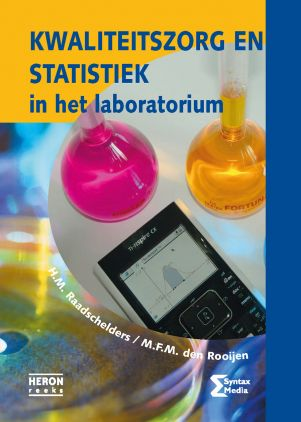
\includegraphics[width=\textwidth]{./afbeeldingen/kwaliteitszorg-statistiek-voorkant} 
\end{figure}
\end{minipage}
\end{block}

Bij dit boek hoort ook een grijs tabellenboekje!

\end{frame}


\begin{frame}{Lesstof}

\begin{block}{Lesstof periode 7}
\begin{itemize}
 \item Hoofdstuk 11
 \item Hoofdstuk 12
 \item Hoofdstuk 13
 \item Hoofdstuk 14 (2 bladzijden, 0 opgaven)
 \item Hoofdstuk 15
\end{itemize}
\end{block}
\end{frame}

\begin{frame}{Toetsen}

\begin{block}{Toetsen periode 7}
\begin{itemize}
 \item Minitoets hoofdstuk 11
 \item Minitoets hoofdstuk 12
 \item Minitoets hoofdstuk 13a
 \item Minitoets hoofdstuk 13b
 \item Minitoets hoofdstuk 15
 \item Eindtoets hoofdstuk 11 t/m hoofdstuk 15
 \end{itemize}
\end{block}
\end{frame}
